% Options for packages loaded elsewhere
% Options for packages loaded elsewhere
\PassOptionsToPackage{unicode}{hyperref}
\PassOptionsToPackage{hyphens}{url}
\PassOptionsToPackage{dvipsnames,svgnames,x11names}{xcolor}
%
\documentclass[
  letterpaper,
  DIV=11,
  numbers=noendperiod]{scrartcl}
\usepackage{xcolor}
\usepackage{amsmath,amssymb}
\setcounter{secnumdepth}{5}
\usepackage{iftex}
\ifPDFTeX
  \usepackage[T1]{fontenc}
  \usepackage[utf8]{inputenc}
  \usepackage{textcomp} % provide euro and other symbols
\else % if luatex or xetex
  \usepackage{unicode-math} % this also loads fontspec
  \defaultfontfeatures{Scale=MatchLowercase}
  \defaultfontfeatures[\rmfamily]{Ligatures=TeX,Scale=1}
\fi
\usepackage{lmodern}
\ifPDFTeX\else
  % xetex/luatex font selection
\fi
% Use upquote if available, for straight quotes in verbatim environments
\IfFileExists{upquote.sty}{\usepackage{upquote}}{}
\IfFileExists{microtype.sty}{% use microtype if available
  \usepackage[]{microtype}
  \UseMicrotypeSet[protrusion]{basicmath} % disable protrusion for tt fonts
}{}
\makeatletter
\@ifundefined{KOMAClassName}{% if non-KOMA class
  \IfFileExists{parskip.sty}{%
    \usepackage{parskip}
  }{% else
    \setlength{\parindent}{0pt}
    \setlength{\parskip}{6pt plus 2pt minus 1pt}}
}{% if KOMA class
  \KOMAoptions{parskip=half}}
\makeatother
% Make \paragraph and \subparagraph free-standing
\makeatletter
\ifx\paragraph\undefined\else
  \let\oldparagraph\paragraph
  \renewcommand{\paragraph}{
    \@ifstar
      \xxxParagraphStar
      \xxxParagraphNoStar
  }
  \newcommand{\xxxParagraphStar}[1]{\oldparagraph*{#1}\mbox{}}
  \newcommand{\xxxParagraphNoStar}[1]{\oldparagraph{#1}\mbox{}}
\fi
\ifx\subparagraph\undefined\else
  \let\oldsubparagraph\subparagraph
  \renewcommand{\subparagraph}{
    \@ifstar
      \xxxSubParagraphStar
      \xxxSubParagraphNoStar
  }
  \newcommand{\xxxSubParagraphStar}[1]{\oldsubparagraph*{#1}\mbox{}}
  \newcommand{\xxxSubParagraphNoStar}[1]{\oldsubparagraph{#1}\mbox{}}
\fi
\makeatother

\usepackage{color}
\usepackage{fancyvrb}
\newcommand{\VerbBar}{|}
\newcommand{\VERB}{\Verb[commandchars=\\\{\}]}
\DefineVerbatimEnvironment{Highlighting}{Verbatim}{commandchars=\\\{\}}
% Add ',fontsize=\small' for more characters per line
\usepackage{framed}
\definecolor{shadecolor}{RGB}{241,243,245}
\newenvironment{Shaded}{\begin{snugshade}}{\end{snugshade}}
\newcommand{\AlertTok}[1]{\textcolor[rgb]{0.68,0.00,0.00}{#1}}
\newcommand{\AnnotationTok}[1]{\textcolor[rgb]{0.37,0.37,0.37}{#1}}
\newcommand{\AttributeTok}[1]{\textcolor[rgb]{0.40,0.45,0.13}{#1}}
\newcommand{\BaseNTok}[1]{\textcolor[rgb]{0.68,0.00,0.00}{#1}}
\newcommand{\BuiltInTok}[1]{\textcolor[rgb]{0.00,0.23,0.31}{#1}}
\newcommand{\CharTok}[1]{\textcolor[rgb]{0.13,0.47,0.30}{#1}}
\newcommand{\CommentTok}[1]{\textcolor[rgb]{0.37,0.37,0.37}{#1}}
\newcommand{\CommentVarTok}[1]{\textcolor[rgb]{0.37,0.37,0.37}{\textit{#1}}}
\newcommand{\ConstantTok}[1]{\textcolor[rgb]{0.56,0.35,0.01}{#1}}
\newcommand{\ControlFlowTok}[1]{\textcolor[rgb]{0.00,0.23,0.31}{\textbf{#1}}}
\newcommand{\DataTypeTok}[1]{\textcolor[rgb]{0.68,0.00,0.00}{#1}}
\newcommand{\DecValTok}[1]{\textcolor[rgb]{0.68,0.00,0.00}{#1}}
\newcommand{\DocumentationTok}[1]{\textcolor[rgb]{0.37,0.37,0.37}{\textit{#1}}}
\newcommand{\ErrorTok}[1]{\textcolor[rgb]{0.68,0.00,0.00}{#1}}
\newcommand{\ExtensionTok}[1]{\textcolor[rgb]{0.00,0.23,0.31}{#1}}
\newcommand{\FloatTok}[1]{\textcolor[rgb]{0.68,0.00,0.00}{#1}}
\newcommand{\FunctionTok}[1]{\textcolor[rgb]{0.28,0.35,0.67}{#1}}
\newcommand{\ImportTok}[1]{\textcolor[rgb]{0.00,0.46,0.62}{#1}}
\newcommand{\InformationTok}[1]{\textcolor[rgb]{0.37,0.37,0.37}{#1}}
\newcommand{\KeywordTok}[1]{\textcolor[rgb]{0.00,0.23,0.31}{\textbf{#1}}}
\newcommand{\NormalTok}[1]{\textcolor[rgb]{0.00,0.23,0.31}{#1}}
\newcommand{\OperatorTok}[1]{\textcolor[rgb]{0.37,0.37,0.37}{#1}}
\newcommand{\OtherTok}[1]{\textcolor[rgb]{0.00,0.23,0.31}{#1}}
\newcommand{\PreprocessorTok}[1]{\textcolor[rgb]{0.68,0.00,0.00}{#1}}
\newcommand{\RegionMarkerTok}[1]{\textcolor[rgb]{0.00,0.23,0.31}{#1}}
\newcommand{\SpecialCharTok}[1]{\textcolor[rgb]{0.37,0.37,0.37}{#1}}
\newcommand{\SpecialStringTok}[1]{\textcolor[rgb]{0.13,0.47,0.30}{#1}}
\newcommand{\StringTok}[1]{\textcolor[rgb]{0.13,0.47,0.30}{#1}}
\newcommand{\VariableTok}[1]{\textcolor[rgb]{0.07,0.07,0.07}{#1}}
\newcommand{\VerbatimStringTok}[1]{\textcolor[rgb]{0.13,0.47,0.30}{#1}}
\newcommand{\WarningTok}[1]{\textcolor[rgb]{0.37,0.37,0.37}{\textit{#1}}}

\usepackage{longtable,booktabs,array}
\newcounter{none} % for unnumbered tables
\usepackage{calc} % for calculating minipage widths
% Correct order of tables after \paragraph or \subparagraph
\usepackage{etoolbox}
\makeatletter
\patchcmd\longtable{\par}{\if@noskipsec\mbox{}\fi\par}{}{}
\makeatother
% Allow footnotes in longtable head/foot
\IfFileExists{footnotehyper.sty}{\usepackage{footnotehyper}}{\usepackage{footnote}}
\makesavenoteenv{longtable}
\usepackage{graphicx}
\makeatletter
\newsavebox\pandoc@box
\newcommand*\pandocbounded[1]{% scales image to fit in text height/width
  \sbox\pandoc@box{#1}%
  \Gscale@div\@tempa{\textheight}{\dimexpr\ht\pandoc@box+\dp\pandoc@box\relax}%
  \Gscale@div\@tempb{\linewidth}{\wd\pandoc@box}%
  \ifdim\@tempb\p@<\@tempa\p@\let\@tempa\@tempb\fi% select the smaller of both
  \ifdim\@tempa\p@<\p@\scalebox{\@tempa}{\usebox\pandoc@box}%
  \else\usebox{\pandoc@box}%
  \fi%
}
% Set default figure placement to htbp
\def\fps@figure{htbp}
\makeatother





\setlength{\emergencystretch}{3em} % prevent overfull lines

\providecommand{\tightlist}{%
  \setlength{\itemsep}{0pt}\setlength{\parskip}{0pt}}



 


\KOMAoption{captions}{tableheading}
\makeatletter
\@ifpackageloaded{caption}{}{\usepackage{caption}}
\AtBeginDocument{%
\ifdefined\contentsname
  \renewcommand*\contentsname{Table of contents}
\else
  \newcommand\contentsname{Table of contents}
\fi
\ifdefined\listfigurename
  \renewcommand*\listfigurename{List of Figures}
\else
  \newcommand\listfigurename{List of Figures}
\fi
\ifdefined\listtablename
  \renewcommand*\listtablename{List of Tables}
\else
  \newcommand\listtablename{List of Tables}
\fi
\ifdefined\figurename
  \renewcommand*\figurename{Figure}
\else
  \newcommand\figurename{Figure}
\fi
\ifdefined\tablename
  \renewcommand*\tablename{Table}
\else
  \newcommand\tablename{Table}
\fi
}
\@ifpackageloaded{float}{}{\usepackage{float}}
\floatstyle{ruled}
\@ifundefined{c@chapter}{\newfloat{codelisting}{h}{lop}}{\newfloat{codelisting}{h}{lop}[chapter]}
\floatname{codelisting}{Listing}
\newcommand*\listoflistings{\listof{codelisting}{List of Listings}}
\makeatother
\makeatletter
\makeatother
\makeatletter
\@ifpackageloaded{caption}{}{\usepackage{caption}}
\@ifpackageloaded{subcaption}{}{\usepackage{subcaption}}
\makeatother
\usepackage{bookmark}
\IfFileExists{xurl.sty}{\usepackage{xurl}}{} % add URL line breaks if available
\urlstyle{same}
\hypersetup{
  pdftitle={IEAP-Rstudio-Series03 Assignment},
  pdfauthor={CLANET Damien; LONG Jiangbin; BINCHE Werner},
  colorlinks=true,
  linkcolor={blue},
  filecolor={Maroon},
  citecolor={Blue},
  urlcolor={Blue},
  pdfcreator={LaTeX via pandoc}}


\title{IEAP-Rstudio-Series03 Assignment}
\author{CLANET Damien \and LONG Jiangbin \and BINCHE Werner}
\date{2026-10-12}
\begin{document}
\maketitle


\section{1. Project Info}\label{project-info}

Our project repository and complete version history can be found on
GitHub:
\href{https://github.com/alonlongsan/IEAP-Series03-RStudio}{IEAP-Series03-RStudio}

\section{2. Introduction and Team
Management}\label{introduction-and-team-management}

\subsection{2.1 Scientific Context}\label{scientific-context}

The objective of this assignment is to reproduce the main results of a
scientific article studying human motor control (Fitts's Law).
Specifically, we aim to investigate whether the effect of Task
Difficulty (ID) on Movement Time (MT) is the same across different
experimental groups (ap, cp, pp). To answer this, we performed data
reorganization, a repeated-measures ANOVA, linear regressions, and
generated publication-ready plots.

\subsection{2.2 Team Management and Git Workflow
Strategy}\label{team-management-and-git-workflow-strategy}

To efficiently collaborate on this project and avoid overriding each
other's work, our team adopted a \textbf{Branch-based Git Workflow}. We
distributed the tasks strategically across different branches:

\begin{itemize}
\tightlist
\item
  \textbf{LONG Jiangbin (\texttt{final\_part\_create\_pdf} branch):}
  Jiangbin was responsible for setting up the main architecture of the
  project. He initialized the GitHub repository, created the master
  Quarto document (\texttt{IEAP-Series03-Rstudio.qmd}), and prepared the
  placeholder structure for the sub-documents.
\item
  \textbf{BINCHE Werner (\texttt{first\_part} branch):} Werner created a
  dedicated branch to handle the data preprocessing. He was in charge of
  using \texttt{tidyverse} to filter out missing data (ID3 and REP3) and
  running the repeated-measures ANOVA using the \texttt{ez} /
  \texttt{rstatix} package.
\item
  \textbf{CLANET Damien (\texttt{ggplot-viz} branch):} Damien worked in
  parallel on the visualization branch. His role was to perform the
  linear regressions for each group and use \texttt{ggplot2} to recreate
  the publication-level graph with the corresponding equations.
\end{itemize}

\textbf{Merge Strategy:} Once our respective sub-documents were complete
and tested locally, we integrated our work into the master Quarto
document via \textbf{Pull Requests / Merging}. This ensured that the
main branch remained stable and successfully rendered the final PDF.

\subsection{2.3 Challenges Encountered and Lessons
Learned}\label{challenges-encountered-and-lessons-learned}

During the execution of this assignment, we encountered several
technical and scientific challenges:

\begin{itemize}
\tightlist
\item
  \textbf{Git Collaboration:} At first, coordinating the merges into the
  master document required careful communication. We learned that
  strictly isolating our code into separate sub-documents
  (\texttt{.qmd}) before pulling and merging is the best way to prevent
  merge conflicts.
\item
  \textbf{Data Reorganization:} We realized that real-world data is
  often messy. The repeated-measures ANOVA requires balanced data.
  Finding and removing the missing data (ID3 in group pp, and REP3)
  using \texttt{dplyr} was a crucial step we had to figure out.
\item
  \textbf{Data Visualization:} Recreating a publication-level graph in
  \texttt{ggplot2} was challenging, especially mathematically
  calculating the linear regression equations for each group separately
  and successfully printing those specific text equations directly onto
  the graph.
\end{itemize}

Working through these challenges significantly improved both our R
programming skills and our practical understanding of version control
using Git.

\begin{center}\rule{0.5\linewidth}{0.5pt}\end{center}

\section{}\label{section}

\begin{Shaded}
\begin{Highlighting}[]
\FunctionTok{library}\NormalTok{(tidyverse)}
\FunctionTok{library}\NormalTok{(ez)}
\end{Highlighting}
\end{Shaded}

\#get the data

\begin{Shaded}
\begin{Highlighting}[]
\CommentTok{\# read a data file that is text with columns separated by spaces and strings as factors}
\NormalTok{results }\OtherTok{\textless{}{-}} \FunctionTok{read.table}\NormalTok{(}\StringTok{"data/Results.txt"}\NormalTok{, }\AttributeTok{header =} \ConstantTok{TRUE}\NormalTok{, }\AttributeTok{sep =} \StringTok{" "}\NormalTok{, }\AttributeTok{stringsAsFactors =} \ConstantTok{TRUE}\NormalTok{)}
\end{Highlighting}
\end{Shaded}

\subsection{Look at the number of measures by GROUP and
ID}\label{look-at-the-number-of-measures-by-group-and-id}

We want a table that shows the number of measures for each combination
og GROUP and ID

\begin{Shaded}
\begin{Highlighting}[]
\NormalTok{results }\SpecialCharTok{\%\textgreater{}\%}
  \FunctionTok{count}\NormalTok{(GROUP, ID )}
\end{Highlighting}
\end{Shaded}

\begin{verbatim}
  GROUP  ID    n
1    ap ID1  740
2    ap ID2  740
3    ap ID3  740
4    cp ID1 1140
5    cp ID2 1140
6    cp ID3 1140
7    pp ID1  760
8    pp ID2  760
9    pp ID3  400
\end{verbatim}

We suppress ID3 and count again

\begin{Shaded}
\begin{Highlighting}[]
\NormalTok{results }\SpecialCharTok{\%\textgreater{}\%}
  \FunctionTok{filter}\NormalTok{(ID }\SpecialCharTok{!=}\StringTok{"ID3"}\NormalTok{) }\SpecialCharTok{\%\textgreater{}\%}
  \FunctionTok{count}\NormalTok{(GROUP, ID ) }
\end{Highlighting}
\end{Shaded}

\begin{verbatim}
  GROUP  ID    n
1    ap ID1  740
2    ap ID2  740
3    cp ID1 1140
4    cp ID2 1140
5    pp ID1  760
6    pp ID2  760
\end{verbatim}

We now check the REP factor

\begin{Shaded}
\begin{Highlighting}[]
\NormalTok{results }\SpecialCharTok{\%\textgreater{}\%}
  \FunctionTok{filter}\NormalTok{(ID }\SpecialCharTok{!=}\StringTok{"ID3"}\NormalTok{) }\SpecialCharTok{\%\textgreater{}\%}
  \FunctionTok{count}\NormalTok{(REP)}
\end{Highlighting}
\end{Shaded}

\begin{verbatim}
  REP    n
1  R1 2040
2  R2 2040
3  R3 1200
\end{verbatim}

\begin{Shaded}
\begin{Highlighting}[]
\NormalTok{results }\SpecialCharTok{\%\textgreater{}\%}
  \FunctionTok{filter}\NormalTok{(ID }\SpecialCharTok{!=} \StringTok{"ID3"}\NormalTok{) }\SpecialCharTok{\%\textgreater{}\%}
  \FunctionTok{count}\NormalTok{(GROUP, REP)}
\end{Highlighting}
\end{Shaded}

\begin{verbatim}
  GROUP REP   n
1    ap  R1 520
2    ap  R2 520
3    ap  R3 440
4    cp  R1 760
5    cp  R2 760
6    cp  R3 760
7    pp  R1 760
8    pp  R2 760
\end{verbatim}

We now suppress REP3 because of missing data and count again

\begin{Shaded}
\begin{Highlighting}[]
\NormalTok{results }\SpecialCharTok{\%\textgreater{}\%}
  \FunctionTok{filter}\NormalTok{(ID }\SpecialCharTok{!=} \StringTok{"ID3"}\NormalTok{) }\SpecialCharTok{\%\textgreater{}\%}
  \FunctionTok{filter}\NormalTok{(REP }\SpecialCharTok{!=} \StringTok{"R3"}\NormalTok{) }\SpecialCharTok{\%\textgreater{}\%}
  \FunctionTok{count}\NormalTok{(GROUP, ID, REP)  }
\end{Highlighting}
\end{Shaded}

\begin{verbatim}
   GROUP  ID REP   n
1     ap ID1  R1 260
2     ap ID1  R2 260
3     ap ID2  R1 260
4     ap ID2  R2 260
5     cp ID1  R1 380
6     cp ID1  R2 380
7     cp ID2  R1 380
8     cp ID2  R2 380
9     pp ID1  R1 380
10    pp ID1  R2 380
11    pp ID2  R1 380
12    pp ID2  R2 380
\end{verbatim}

\begin{Shaded}
\begin{Highlighting}[]
\CommentTok{\# count the number of participants in each group after suppressing ID3 and REP3}
\NormalTok{results }\SpecialCharTok{\%\textgreater{}\%}
  \FunctionTok{filter}\NormalTok{(ID }\SpecialCharTok{!=} \StringTok{"ID3"}\NormalTok{) }\SpecialCharTok{\%\textgreater{}\%}
  \FunctionTok{filter}\NormalTok{(REP }\SpecialCharTok{!=} \StringTok{"R3"}\NormalTok{) }\SpecialCharTok{\%\textgreater{}\%}
  \FunctionTok{count}\NormalTok{(GROUP) }
\end{Highlighting}
\end{Shaded}

\begin{verbatim}
  GROUP    n
1    ap 1040
2    cp 1520
3    pp 1520
\end{verbatim}

\begin{Shaded}
\begin{Highlighting}[]
\CommentTok{\# count how many different SUBJ by GROUP}
\NormalTok{results }\SpecialCharTok{\%\textgreater{}\%}
  \FunctionTok{filter}\NormalTok{(ID }\SpecialCharTok{!=} \StringTok{"ID3"}\NormalTok{) }\SpecialCharTok{\%\textgreater{}\%}
  \FunctionTok{filter}\NormalTok{(REP }\SpecialCharTok{!=} \StringTok{"R3"}\NormalTok{) }\SpecialCharTok{\%\textgreater{}\%}
  \FunctionTok{group\_by}\NormalTok{(GROUP) }\SpecialCharTok{\%\textgreater{}\%}
  \FunctionTok{summarise}\NormalTok{(}\AttributeTok{n\_subj =} \FunctionTok{n\_distinct}\NormalTok{(SUBJ))}
\end{Highlighting}
\end{Shaded}

\begin{verbatim}
# A tibble: 3 x 2
  GROUP n_subj
  <fct>  <int>
1 ap        13
2 cp        19
3 pp        19
\end{verbatim}

We have created a clean data set

\begin{Shaded}
\begin{Highlighting}[]
\CommentTok{\# Create a clean data set}
\NormalTok{clean\_results }\OtherTok{\textless{}{-}}\NormalTok{ results }\SpecialCharTok{\%\textgreater{}\%}
  \FunctionTok{filter}\NormalTok{(ID }\SpecialCharTok{!=} \StringTok{"ID3"}\NormalTok{) }\SpecialCharTok{\%\textgreater{}\%}
  \FunctionTok{filter}\NormalTok{(REP }\SpecialCharTok{!=} \StringTok{"R3"}\NormalTok{) }\SpecialCharTok{\%\textgreater{}\%}
  \FunctionTok{droplevels}\NormalTok{()}

\CommentTok{\# Check the clean data set}
\FunctionTok{head}\NormalTok{(clean\_results)}
\end{Highlighting}
\end{Shaded}

\begin{verbatim}
  GROUP  SUBJ TRIAL ORI     DIR  ID REP NbVelPeaks MovementTime
1    ap apS01   T01   W outward ID1  R1          2         1.23
2    ap apS01   T01   W  inward ID1  R1          2         1.26
3    ap apS01   T01  NW outward ID1  R1          3         1.14
4    ap apS01   T01  NW  inward ID1  R1          2         0.90
5    ap apS01   T01   N outward ID1  R1          3         1.11
6    ap apS01   T01   N  inward ID1  R1          3         0.81
\end{verbatim}

\begin{Shaded}
\begin{Highlighting}[]
\FunctionTok{count}\NormalTok{(clean\_results, GROUP)}
\end{Highlighting}
\end{Shaded}

\begin{verbatim}
  GROUP    n
1    ap 1040
2    cp 1520
3    pp 1520
\end{verbatim}

\begin{Shaded}
\begin{Highlighting}[]
\FunctionTok{count}\NormalTok{(clean\_results, GROUP, ID, REP)}
\end{Highlighting}
\end{Shaded}

\begin{verbatim}
   GROUP  ID REP   n
1     ap ID1  R1 260
2     ap ID1  R2 260
3     ap ID2  R1 260
4     ap ID2  R2 260
5     cp ID1  R1 380
6     cp ID1  R2 380
7     cp ID2  R1 380
8     cp ID2  R2 380
9     pp ID1  R1 380
10    pp ID1  R2 380
11    pp ID2  R1 380
12    pp ID2  R2 380
\end{verbatim}

\begin{Shaded}
\begin{Highlighting}[]
\NormalTok{ANOVA }\OtherTok{\textless{}{-}} \FunctionTok{ezANOVA}\NormalTok{(}
  \AttributeTok{data =}\NormalTok{ clean\_results,}
  \AttributeTok{dv =}\NormalTok{ .(MovementTime),}
  \AttributeTok{wid =}\NormalTok{ .(SUBJ),}
  \AttributeTok{within =}\NormalTok{ .(ID),}
  \AttributeTok{between =}\NormalTok{ .(GROUP),}
  \AttributeTok{type =} \DecValTok{3}
\NormalTok{)}
\end{Highlighting}
\end{Shaded}

\begin{verbatim}
Warning: Data is unbalanced (unequal N per group). Make sure you specified a
well-considered value for the type argument to ezANOVA().
\end{verbatim}

\begin{verbatim}
Warning: Collapsing data to cell means. *IF* the requested effects are a subset
of the full design, you must use the "within_full" argument, else results may
be inaccurate.
\end{verbatim}

\begin{Shaded}
\begin{Highlighting}[]
\NormalTok{ANOVA}
\end{Highlighting}
\end{Shaded}

\begin{verbatim}
$ANOVA
    Effect DFn DFd        F            p p<.05        ges
2    GROUP   2  48 37.24408 1.720007e-10     * 0.57462110
3       ID   1  48 26.10886 5.543011e-06     * 0.06581307
4 GROUP:ID   2  48 11.58124 7.866206e-05     * 0.05882293
\end{verbatim}

\begin{Shaded}
\begin{Highlighting}[]
\FunctionTok{library}\NormalTok{(ggplot2)}
\CommentTok{\# plot the interaction between GROUP and ID and add error bars containing the }
\CommentTok{\# within (group x ID) standard deviation around the mean}
\NormalTok{interaction\_plot\_Group\_ID }\OtherTok{\textless{}{-}} \FunctionTok{ggplot}\NormalTok{(clean\_results) }\SpecialCharTok{+}
  \FunctionTok{aes}\NormalTok{(}\AttributeTok{x =}\NormalTok{ ID, }\AttributeTok{y =}\NormalTok{ MovementTime, }\AttributeTok{color =}\NormalTok{ GROUP) }\SpecialCharTok{+}
  \FunctionTok{stat\_summary}\NormalTok{(}\AttributeTok{fun =}\NormalTok{ mean, }\AttributeTok{geom =} \StringTok{"line"}\NormalTok{, }\FunctionTok{aes}\NormalTok{(}\AttributeTok{group =}\NormalTok{ GROUP)) }\SpecialCharTok{+}
  \FunctionTok{stat\_summary}\NormalTok{(}\AttributeTok{fun.data =}\NormalTok{ mean\_sdl, }\AttributeTok{fun.args =} \FunctionTok{list}\NormalTok{(}\AttributeTok{mult =}\NormalTok{ .}\DecValTok{5}\NormalTok{), }\AttributeTok{geom =} \StringTok{"errorbar"}\NormalTok{, }\AttributeTok{width =} \FloatTok{0.01}\NormalTok{) }\SpecialCharTok{+}
  \FunctionTok{stat\_summary}\NormalTok{(}\AttributeTok{fun =}\NormalTok{ mean, }\AttributeTok{geom =} \StringTok{"point"}\NormalTok{, }\AttributeTok{shape=} \DecValTok{21}\NormalTok{, }\AttributeTok{fill =} \StringTok{"white"}\NormalTok{, }\AttributeTok{size =} \DecValTok{3}\NormalTok{) }\SpecialCharTok{+}
  \FunctionTok{labs}\NormalTok{(}\AttributeTok{title =} \StringTok{"Interaction between GROUP and ID on MovementTime"}\NormalTok{,}
       \AttributeTok{x =} \StringTok{"ID"}\NormalTok{,}
       \AttributeTok{y =} \StringTok{"Mean MovementTime (s)"}\NormalTok{) }\SpecialCharTok{+}
  \FunctionTok{theme\_minimal}\NormalTok{()}

\FunctionTok{show}\NormalTok{(interaction\_plot\_Group\_ID)}
\end{Highlighting}
\end{Shaded}

\pandocbounded{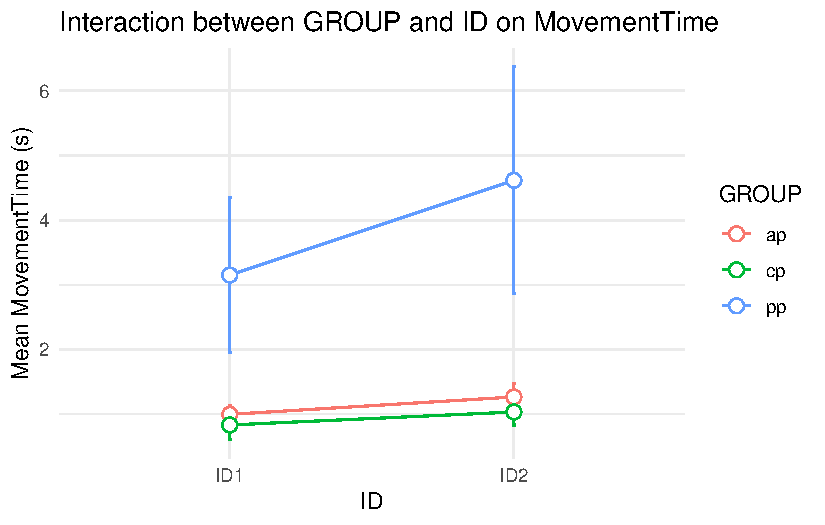
\includegraphics[keepaspectratio]{IEAP-Series03-Rstudio_files/figure-pdf/unnamed-chunk-6-1.pdf}}

\begin{Shaded}
\begin{Highlighting}[]
\NormalTok{clean\_results }\OtherTok{\textless{}{-}}\NormalTok{ clean\_results }\SpecialCharTok{\%\textgreater{}\%}
  \FunctionTok{mutate}\NormalTok{(}\AttributeTok{ID\_num =} \FunctionTok{as.numeric}\NormalTok{(}\FunctionTok{factor}\NormalTok{(ID)))}

\ControlFlowTok{for}\NormalTok{ (g }\ControlFlowTok{in} \FunctionTok{levels}\NormalTok{(clean\_results}\SpecialCharTok{$}\NormalTok{GROUP)) \{}
\NormalTok{  d }\OtherTok{\textless{}{-}} \FunctionTok{filter}\NormalTok{(clean\_results, GROUP }\SpecialCharTok{==}\NormalTok{ g)}
\NormalTok{  model }\OtherTok{\textless{}{-}} \FunctionTok{lm}\NormalTok{(MovementTime }\SpecialCharTok{\textasciitilde{}}\NormalTok{ ID\_num, }\AttributeTok{data =}\NormalTok{ d)}

  \FunctionTok{cat}\NormalTok{(g, }\StringTok{": MT ="}\NormalTok{,}
      \FunctionTok{round}\NormalTok{(}\FunctionTok{coef}\NormalTok{(model)[}\DecValTok{1}\NormalTok{], }\DecValTok{3}\NormalTok{), }\StringTok{"+"}\NormalTok{,}
      \FunctionTok{round}\NormalTok{(}\FunctionTok{coef}\NormalTok{(model)[}\DecValTok{2}\NormalTok{], }\DecValTok{3}\NormalTok{), }\StringTok{"* ID}\SpecialCharTok{\textbackslash{}n}\StringTok{"}\NormalTok{)}
\NormalTok{\}}
\end{Highlighting}
\end{Shaded}

\begin{verbatim}
ap : MT = 0.73 + 0.269 * ID
cp : MT = 0.634 + 0.201 * ID
pp : MT = 1.689 + 1.464 * ID
\end{verbatim}

\section{1.5 Save a graph in a PDF file for
publication}\label{save-a-graph-in-a-pdf-file-for-publication}

\begin{Shaded}
\begin{Highlighting}[]
\CommentTok{\# Équations de régression par GROUP (calculées, pas écrites à la main)}
\NormalTok{eq }\OtherTok{\textless{}{-}}\NormalTok{ clean\_results }\SpecialCharTok{\%\textgreater{}\%}
  \FunctionTok{group\_by}\NormalTok{(GROUP) }\SpecialCharTok{\%\textgreater{}\%}
  \FunctionTok{group\_modify}\NormalTok{(}\SpecialCharTok{\textasciitilde{}}\NormalTok{ \{}
\NormalTok{    m }\OtherTok{\textless{}{-}} \FunctionTok{lm}\NormalTok{(MovementTime }\SpecialCharTok{\textasciitilde{}}\NormalTok{ ID\_num, }\AttributeTok{data =}\NormalTok{ .x)}
    \FunctionTok{tibble}\NormalTok{(}\AttributeTok{intercept =} \FunctionTok{coef}\NormalTok{(m)[}\DecValTok{1}\NormalTok{], }\AttributeTok{slope =} \FunctionTok{coef}\NormalTok{(m)[}\DecValTok{2}\NormalTok{])}
\NormalTok{  \}) }\SpecialCharTok{\%\textgreater{}\%}
  \FunctionTok{ungroup}\NormalTok{() }\SpecialCharTok{\%\textgreater{}\%}
  \FunctionTok{mutate}\NormalTok{(}\AttributeTok{label =} \FunctionTok{sprintf}\NormalTok{(}\StringTok{"\%s: MT = \%.3f + \%.3f * ID"}\NormalTok{, GROUP, intercept, slope))}

\CommentTok{\# Limites des axes et position des équations (en haut à gauche, empilées)}
\NormalTok{y\_max }\OtherTok{\textless{}{-}} \FunctionTok{max}\NormalTok{(clean\_results}\SpecialCharTok{$}\NormalTok{MovementTime, }\AttributeTok{na.rm =} \ConstantTok{TRUE}\NormalTok{)}
\NormalTok{eq }\OtherTok{\textless{}{-}}\NormalTok{ eq }\SpecialCharTok{\%\textgreater{}\%}
  \FunctionTok{mutate}\NormalTok{(}\AttributeTok{x =} \FloatTok{0.55}\NormalTok{,}
         \AttributeTok{y =}\NormalTok{ y\_max }\SpecialCharTok{*}\NormalTok{ (}\FloatTok{0.98} \SpecialCharTok{{-}} \FloatTok{0.07} \SpecialCharTok{*}\NormalTok{ (}\FunctionTok{row\_number}\NormalTok{() }\SpecialCharTok{{-}} \DecValTok{1}\NormalTok{)))}

\NormalTok{fig3 }\OtherTok{\textless{}{-}} \FunctionTok{ggplot}\NormalTok{(clean\_results, }\FunctionTok{aes}\NormalTok{(}\AttributeTok{x =}\NormalTok{ ID\_num, }\AttributeTok{y =}\NormalTok{ MovementTime, }\AttributeTok{color =}\NormalTok{ GROUP)) }\SpecialCharTok{+}
  \CommentTok{\# moyenne +/{-} 0.5 SD pour chaque GROUP x ID}
  \FunctionTok{stat\_summary}\NormalTok{(}\AttributeTok{fun.data =}\NormalTok{ mean\_sdl, }\AttributeTok{fun.args =} \FunctionTok{list}\NormalTok{(}\AttributeTok{mult =}\NormalTok{ .}\DecValTok{5}\NormalTok{),}
               \AttributeTok{geom =} \StringTok{"errorbar"}\NormalTok{, }\AttributeTok{width =} \FloatTok{0.03}\NormalTok{) }\SpecialCharTok{+}
  \FunctionTok{stat\_summary}\NormalTok{(}\AttributeTok{fun =}\NormalTok{ mean, }\AttributeTok{geom =} \StringTok{"point"}\NormalTok{, }\AttributeTok{shape =} \DecValTok{21}\NormalTok{, }\AttributeTok{fill =} \StringTok{"white"}\NormalTok{, }\AttributeTok{size =} \DecValTok{3}\NormalTok{) }\SpecialCharTok{+}
  \CommentTok{\# droites de régression par GROUP}
  \FunctionTok{geom\_smooth}\NormalTok{(}\AttributeTok{method =} \StringTok{"lm"}\NormalTok{, }\AttributeTok{se =} \ConstantTok{FALSE}\NormalTok{, }\AttributeTok{fullrange =} \ConstantTok{TRUE}\NormalTok{, }\AttributeTok{linewidth =} \FloatTok{0.8}\NormalTok{) }\SpecialCharTok{+}
  \CommentTok{\# équations sur le graphique}
  \FunctionTok{geom\_text}\NormalTok{(}\AttributeTok{data =}\NormalTok{ eq, }\FunctionTok{aes}\NormalTok{(}\AttributeTok{x =}\NormalTok{ x, }\AttributeTok{y =}\NormalTok{ y, }\AttributeTok{label =}\NormalTok{ label, }\AttributeTok{color =}\NormalTok{ GROUP),}
            \AttributeTok{hjust =} \DecValTok{0}\NormalTok{, }\AttributeTok{size =} \FloatTok{3.5}\NormalTok{, }\AttributeTok{inherit.aes =} \ConstantTok{FALSE}\NormalTok{, }\AttributeTok{show.legend =} \ConstantTok{FALSE}\NormalTok{) }\SpecialCharTok{+}
  \CommentTok{\# geom\_blank pour forcer les limites des axes}
  \FunctionTok{geom\_blank}\NormalTok{(}\AttributeTok{data =} \FunctionTok{tibble}\NormalTok{(}\AttributeTok{ID\_num =} \FunctionTok{c}\NormalTok{(}\FloatTok{0.5}\NormalTok{, }\FloatTok{2.5}\NormalTok{), }\AttributeTok{MovementTime =} \FunctionTok{c}\NormalTok{(}\DecValTok{0}\NormalTok{, y\_max)),}
             \FunctionTok{aes}\NormalTok{(}\AttributeTok{x =}\NormalTok{ ID\_num, }\AttributeTok{y =}\NormalTok{ MovementTime), }\AttributeTok{inherit.aes =} \ConstantTok{FALSE}\NormalTok{) }\SpecialCharTok{+}
  \FunctionTok{scale\_x\_continuous}\NormalTok{(}\AttributeTok{breaks =} \FunctionTok{seq\_along}\NormalTok{(}\FunctionTok{levels}\NormalTok{(clean\_results}\SpecialCharTok{$}\NormalTok{ID)),}
                     \AttributeTok{labels =} \FunctionTok{levels}\NormalTok{(clean\_results}\SpecialCharTok{$}\NormalTok{ID)) }\SpecialCharTok{+}
  \FunctionTok{labs}\NormalTok{(}\AttributeTok{x =} \StringTok{"Index of difficulty (ID)"}\NormalTok{,}
       \AttributeTok{y =} \StringTok{"Movement time (s)"}\NormalTok{,}
       \AttributeTok{color =} \StringTok{"Group"}\NormalTok{) }\SpecialCharTok{+}
  \FunctionTok{theme\_classic}\NormalTok{(}\AttributeTok{base\_size =} \DecValTok{12}\NormalTok{)}

\NormalTok{fig3}
\end{Highlighting}
\end{Shaded}

\begin{verbatim}
`geom_smooth()` using formula = 'y ~ x'
\end{verbatim}

\pandocbounded{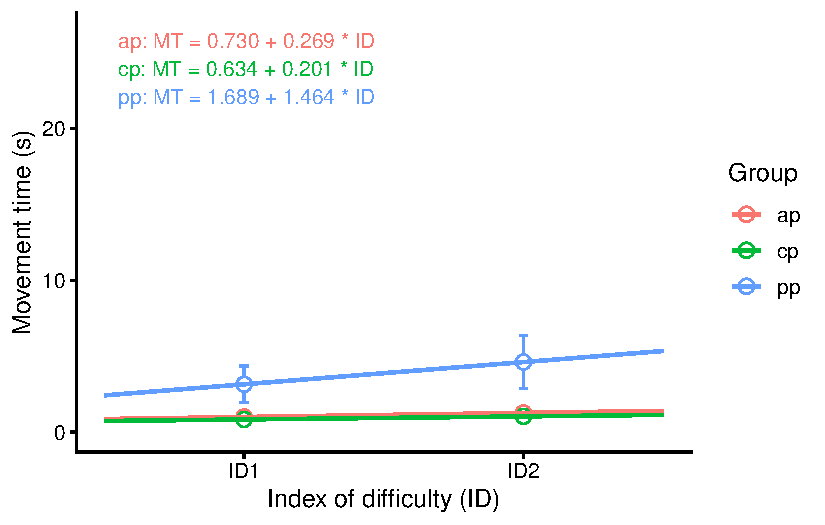
\includegraphics[keepaspectratio]{IEAP-Series03-Rstudio_files/figure-pdf/fig3-plot-1.pdf}}

\section{1.6 Export the graph as a PDF file for
publication}\label{export-the-graph-as-a-pdf-file-for-publication}

\begin{Shaded}
\begin{Highlighting}[]
\FunctionTok{ggsave}\NormalTok{(}\StringTok{"Fig3\_MovementTime\_ID.pdf"}\NormalTok{, }\AttributeTok{plot =}\NormalTok{ fig3,}
       \AttributeTok{width =} \DecValTok{8}\NormalTok{, }\AttributeTok{height =} \DecValTok{6}\NormalTok{, }\AttributeTok{units =} \StringTok{"in"}\NormalTok{, }\AttributeTok{device =}\NormalTok{ cairo\_pdf)}
\end{Highlighting}
\end{Shaded}

\begin{verbatim}
`geom_smooth()` using formula = 'y ~ x'
\end{verbatim}

\section{1.7 Differences with the
article}\label{differences-with-the-article}

My results lead to the same conclusion as the article: the effect of
difficulty (ID) on movement time is not the same in all groups. It is
much stronger in patients (group pp) than in the two control groups,
which corresponds to the significant GROUP × ID interaction, F(2, 48) =
11.58, p \textless{} .001. The degrees of freedom (2, 48) are the same
as in the article, so we are working on the same sample. The mean
movement times are also close to those in the figure: in patients, I get
about 3.15 s and 4.62 s for ID = 3.8 and 5.43 bits, compared with about
3 s and 4 s in the article.

However, the regression lines are not exactly the same. My slopes are
steeper than those in the article (0.898 vs 0.672 for patients, 0.165 vs
0.118 for the age-matched group, 0.123 vs 0.097 for the young group).
The intercept for patients is also negative in my analysis (-0.259),
whereas in the article the three lines meet close to ID = 0.

I think this comes from the simplified method. I removed ID3 and REP3 to
get complete data, so only two levels of ID remain. Each line therefore
passes exactly through two means, and the intercept is an extrapolation
far from the data: a small difference in the means changes the result a
lot. With only two points, we also cannot check that the relationship is
really linear. In addition, I worked with trial means, which are
sensitive to extreme values in patients (up to 26 s), whereas the
article used a more sophisticated method.

In conclusion, the simplified method is sufficient to answer the initial
question (is the effect of difficulty the same in all groups?), but it
does not allow a precise estimate of the slope and intercept of Fitts'
law.

\section{Appendices}\label{appendices}

\subsection{Data Sources}\label{data-sources}

The dataset used in this analysis is \texttt{Results.txt}, which was
provided by the professor for this assignment.

\subsection{Scientific References}\label{scientific-references}

\begin{itemize}
\tightlist
\item
  Mottet, D., van Dokkum, L. E. H., Froger, J., Gouaïch, A., \& Laffont,
  I. (2017). Trajectory formation principles are the same after mild or
  moderate stroke. \emph{PLoS ONE}, 12(3): e0173674. DOI:
  \href{https://journals.plos.org/plosone/article?id=10.1371/journal.pone.0173674}{10.1371/journal.pone.0173674}
\end{itemize}

\begin{center}\rule{0.5\linewidth}{0.5pt}\end{center}

\section{Grading Checklist}\label{grading-checklist}

\begin{itemize}
\tightlist
\item[$\boxtimes$]
  README.md file exists and is clear.
\item[$\boxtimes$]
  LICENSE file exists.
\item[$\boxtimes$]
  IEAP-Series03-Rstudio.qmd (the master document) is complete.
\item[$\boxtimes$]
  The corresponding PDF file is successfully generated.
\item[$\boxtimes$]
  A clear git history, with meaningful commit messages.
\item[$\boxtimes$]
  At least one commit per question of the report.
\item[$\boxtimes$]
  A principled use of branches for parallel work.
\end{itemize}




\end{document}
